\documentclass{report}
\usepackage[utf8]{inputenc}
\usepackage[spanish]{babel}
\usepackage{graphicx}
\usepackage{listings}
\usepackage{xcolor}

\lstset{
	breaklines=true,
	postbreak=\mbox{\textcolor{red}{$\hookrightarrow$}\space},
	}

\title{Vectorizado de siluetas con algoritmo genético}
\author{Adrián Arroyo Calle}
\date{ Octubre-Noviembre 2018}
\begin{document}

\maketitle

\chapter{Introducción}
En el mundo gráfico existen dos tipos fundamentales de imágenes.
En primer lugar tenemos las rasterizadas, donde se almacena la información de cada píxel de forma individual.
Estas imágenes son las generadas por escáneres y cámaras fotográficas, así como por renders
de ordenador. Los formatos más usados son JPEG y PNG. En segundo lugar tenemos las imágenes
vectoriales, donde se almacenan funciones matemáticas, que en el momento de su visualización son calculadas. 
Este tipo de imágenes son muy usadas en ilustraciones y diseño gráfico, ya que no pierden calidad. Los formatos más usados son SVG y AI. 

Para obtener una imagen rasterizada desde una imagen vectorial, el procedimiento es
sencillo. Simplmente se aplican las fórmulas matemáticas sobre un lienzo de un determinado
tamaño. En cambio, el procedimiento inverso es extremadamente complicado. 

El algoritmo genético presentado en este documento permite transformar imágenes rasterizadas
sencillas, en blanco y negro, en imágenes vectoriales.

\chapter{Estructura general}

El procedimiento básico que seguirá el programa, que será implementado en el lenguaje 
de programación Rust\cite{Matsakis:2014:RL:2692956.2663188}, será el siguiente:

\begin{enumerate}
	\item Leer imagen rasterizada de entrada
	\item Pasar la imagen a escala de grises
	\item Detección de esquinas en la imagen
	\item Optimización de las conexiones entre esquinas
	\item Salida de la imagen vectorial
\end{enumerate}

Para los 3 primeros pasos usaremos librerías de código abierto disponibles para Rust. Concretamente
usaremos image e imageproc. Esta última contiene los algoritmos de detección de esquinas FAST9 y 
FAST12. Sin embargo posteriormente se comprobó que ambos algoritmos tenían tasas de acierto
demasiado bajas y por ello se permite la edición manual de las esquinas.

Será en el paso 4 es donde se aplicará el algoritmo genético, ya que se trata de una tarea de 
optimización. Los algoritmos genéticos pueden ser aplicados de forma exitosa en problemas donde 
necesitemos optimizar algo. En nuestro caso, queremos optimizar el trazado de una línea a que 
respete la forma original sobre la que se está dibujando. Esta línea será una curva cúbica de Bézier.

Finalmente el último paso se realizará de forma trivial por nosotros mismos, 
exportando la imagen a SVG, un formato estándar de gráficos vectoriales.

\chapter{Detección de esquinas}
La librería imageproc contiene los algoritmos de detección de esquinas
FAST9 y FAST12 \cite{rosten_2006_machine} (acrónimo de Features from accelerated segment test). 
Estos algoritmos, son mucho más rápidos que el
 famoso algoritmo de Harris-Stephens, ofreciendo una calidad aceptable, aunque no suficiente para 
 nuestro algoritmo de vectorización. Un ejemplo de su funcionamiento lo podemos ver en la 
 figura \ref{fig:fast-png}.

 % EXPLICAR FAST

\section{Interfaz de usuario}

Debido a la baja tasa de aciertos de FAST9 y FAST12 en las imágenes de prueba, se permite también
añadir puntos de forma manual. Para ello se ha diseñado una interfaz gráfica en GTK3, gracias a
la librería gtk-rs que permite usar GTK en Rust. La interfaz fue diseñada en Glade. La interfaz, 
que se aprecia en la figura \ref{fig:interfaz}, 
es muy sencilla. El funcionamiento principal es con el ratón. Cuando se hace click izquierdo en un
lugar de la imagen se añade una esquina. Es importante tener en cuenta el orden en el que se añaden las esquinas
ya que cada esquina buscará una curva que la una con la esquina añadida inmediatamente antes.
Además hay varios botones en el lateral derecho. Un botón para aplicar FAST9 a la imagen \ref{fig:fast9}, otro para eliminar 
todas las esquinas y otro para ejecutar el algoritmo.

\begin{figure}
	\center{
		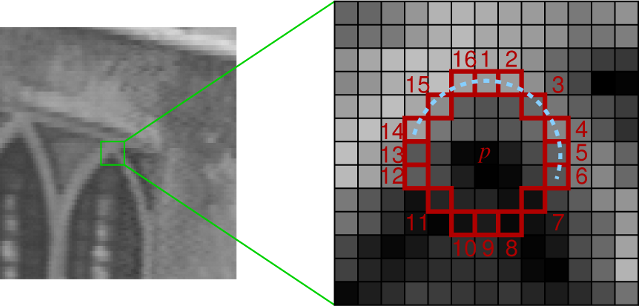
\includegraphics[width=\textwidth]{fast.png}
	}
	\caption{\label{fig:fast-png} Ejemplo de ejecución de FAST sobre una imagen}
\end{figure}

\begin{figure}
	\center{
		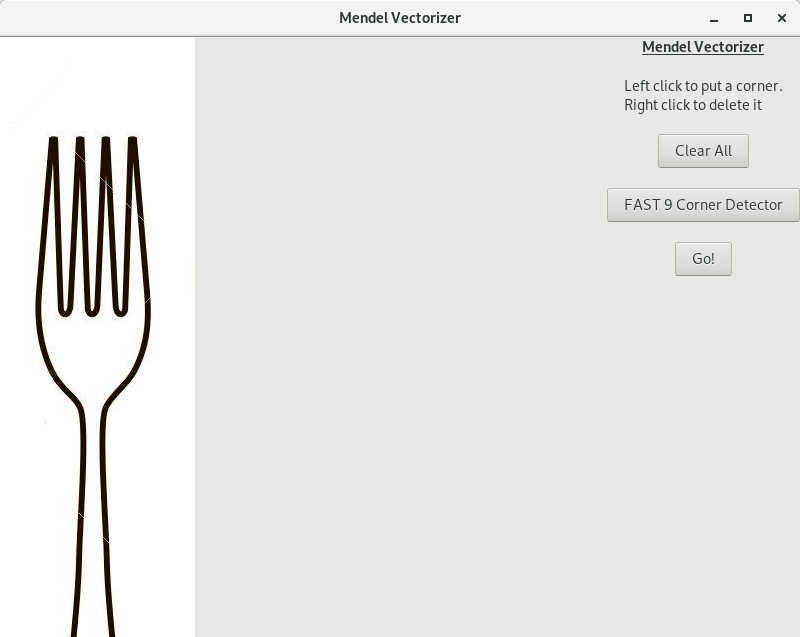
\includegraphics[width=\textwidth]{interfaz-usuario.png}
	}
	\caption{\label{fig:interfaz} Interfaz de usuario para seleccionar esquinas}
\end{figure}

\begin{figure}
	\center{
		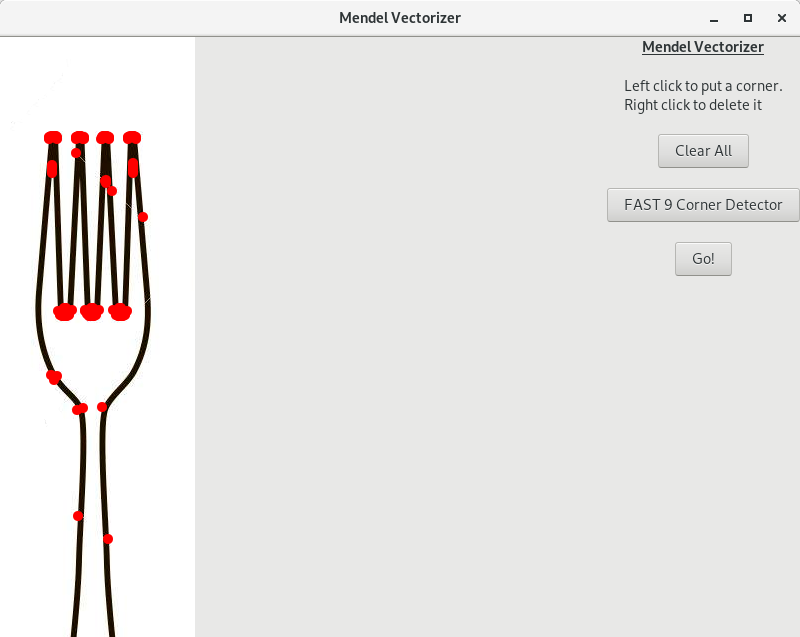
\includegraphics[width=\textwidth]{fast9.png}
	}
	\caption{\label{fig:fast9} Ejemplo de ejecución de FAST9 en la interfaz de usuario}
\end{figure}

\chapter{Algoritmo genético}

Los algoritmos genéticos son aquellos que se basan en el concepto de la evolución biológica.
En estos algoritmo se crea una muestra con parámetros aleatorios y se evalúa su desempeño.
Los peores son eliminados y los mejores son recombinados y sufren mutaciones aleatorias. Así de forma repetitiva hasta
llegar a tener una muestra con parámetros suficientemente buenos como para resolver el problema de 
forma casi óptima.

\section{Curva cúbica de Bézier}

El algoritmo en esencia trata de encontrar una línea que una dos puntos, de forma lo más parecida
posible a una imagen dada. Estas líneas en nuestro caso van a ser siempre curvas cúbicas de Bézier,
un subtipo de spline muy usado en gráficos por ordenador.\cite{wiki:bezier}

Estas curvas se basan en dos puntos de inicio y final y dos puntos de control, que permiten controlar
la curva con facilidad, véase la figura \ref{fig:bezier}.

\begin{figure}
	\center{
		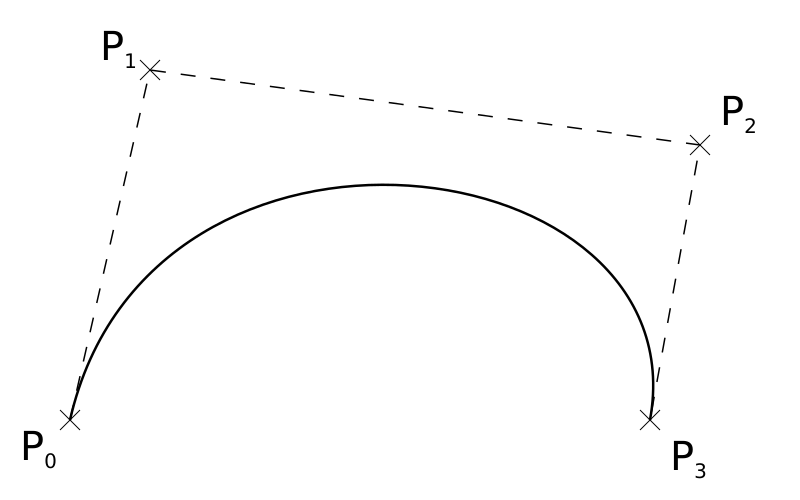
\includegraphics[width=\textwidth]{bezier.png}
	}
	\caption{\label{fig:bezier} Curva cúbica de Bézier}
\end{figure}

La forma paramétrica de una curva cúbica de Bézier es la siguiente:  \\

\begin{math}
	\mathbf{B}(t)=\mathbf{P}_0(1-t)^3+3\mathbf{P}_1t(1-t)^2+3\mathbf{P}_2t^2(1-t)+\mathbf{P}_3t^3 \mbox{ , } t \in [0,1].
\end{math}

Nuestras curvas siempre van a tener como punto de inicio y punto final las esquinas que se tratan de unir, los únicos
puntos que sufren modificaciones son los puntos de control. Estos puntos se definen por sus coordenadas cartesianas. Por ello, en cada curva hay 4 valores reales a optimizar.

\section{Función de evaluación}

Un ingrediente fundamental del algoritmo genético es la función de evaluación, que mide cuán buena
es la solución dada por un individuo. Nuestra función de evaluación toma la curva cúbica de Bezier y 
calcula
los puntos en 100 lugares de la curva. Estos puntos se comparan con la imagen real, si ahí había una línea
se suma un punto, si no, se resta 100. De este modo se penaliza gravemente salirse de la curva. Esto se hace así ya que la otra opción
evidente (bonificar mantenerse en la línea) podría dar lugar a resultados inesperados. 

Pongamos como ejemplo una función de evaluación que bonifique por estar sobre la línea y no penalice por salirse de esta. Una línea bien adaptada a estas condiciones podría recorrerse toda la imagen, cruzando todas las líneas posibles, generando un garabato totalmente inútil pero muy bueno según esta función. Por ello, nuestra función de evaluación se basa en penalizar las salidas de la línea.

La función de evaluación presentada no es perfecta, ya que puede pasar de largo el punto final y dar la vuelta. Esta curva es más larga que la óptima, pero al estar completamente dentro de la línea negra original, la función de evaluación no la puede clasificar como peor que otras alternativas.
Para solventar este problema se propuso que la longitud de la curva tuviese una implicación en la función. No obstante, el cálculo de la longitud de
una curva de Bezier es demasiado complejo y se ha optado por ignorar esta posible mejora.

\subsection{Pseudocódigo}

\begin{lstlisting}
function evaluar(imagen,curva) {
	score <- 0
	for i in 0..100 {
		punto <- calcular_punto(curva,i)
		pixel <- imagen(punto)
		if(pixel is not black){
			score <- score - 100
		}
	}
	return score
}
\end{lstlisting}

Tanto la operación del cálculo de punto, como obtener el pixel de la imagen son constantes. Al ser un bucle que se ejecuta siempre 100 veces, toda la función de evaluación es constante, es decir, $ O(1) $.

\section{Selección natural}

La función de selección natural deja únicamente las 500 mejores curvas, de acuerdo a la función de evaluación, es decir, las mejor adaptadas de momento. Para la ordenación, Rust usa
un algoritmo denominado Timsort, una variante de Mergesort que mejora el mejor caso, pero en promedio sigue siendo $ O(n\log{n}) $. 

\begin{lstlisting}
function seleccion_natural(imagen,poblacion) {
	poblacion <- ordenar(poblacion,evaluar(imagen))
	return poblacion[0..500]
}
\end{lstlisting}

\section{Población inicial}
La población inicial se forma con 1000 curvas generadas con parámetros totalmente aleatorios. Los valores de cada coordenada, eso sí, están 
comprendidos entre $-d$ y $d$ siendo $d$ la distancia en línea recta entre los puntos de inicio y final.

\begin{lstlisting}
function inicial(){
	for i in 0..1000 {
		puntoA <- puntoAleatorio()
		puntoB <- puntoAleatorio()
	}
	return curva(puntoA,puntoB)
}
\end{lstlisting}

Esta generación inicial tiene una complejidad constante, ya que el bucle siempre es igual de largo. Por tanto, $ O(1) $.

\section{Recombinación}

El proceso de recombinación permite mezclar los mejores especímenes tratando de conseguir uno mejor. Este algoritmo genético es de tipo
RCGA (Real Coded Genetic Algorithm) ya que los genes son números reales, en contraposición a los típicos genes binarios.

Para estos algoritmos existen distintas variantes, aquí se usa el sistema de blend. El sistema de blend implica que de entre los dos padres
se toman los valores mínimos y máximos para cada coordenada. Posteriormente se elige un nuevo valor de forma aleatoria con la condición de que 
esté dentro del rango de mínimo y máximo definido anteriormente.

\begin{lstlisting}
function recombinacion(poblacion){
	for i in 0..250 {
		minXA <- min(poblacion[i].A.X,poblacion[i+1].A.X)
		maxXA <- min(poblacion[i].A.X,poblacion[i+1].A.X)
		...

		XA <- random(minXA,maxXA)
		...

		poblacion.add(curva(XA,YA,XB,YB))
	}
}
\end{lstlisting}

La complejidad de la recombinación también es constante ya que el bucle siempre se ejecuta para 250 parejas. Las operaciones dentro del bucle son
todas constantes también. Por tanto: $ O(1) $.

\section{Mutación}

La fase de mutación permite generar pequeñas variaciones aleatorias respecto a la población. Afecta al 25\% de la población (una tasa algo elevada en algoritmos genéticos) aunque solo afecta a una coordenada a la vez. 

Al ser un algoritmo RCGA, no vale simplemente con cambiar el valor de un bit. El enfoque utilizado en este algoritmo es el de una distribución normal de cambios. La distribución tiene la forma $ N(0,\frac{d/2}) $. Esto implica que en la mayoría de las ocasiones la variación (tanto positiva como negativa) en la coordenada será bastante pequeña.

\begin{lstlisting}
function mutacion(poblacion){
	for curva in poblacion {
		if ( mutacion ) {
			cambio <- random(0,4)
			variacion <- normal(0,d/2)
			switch(cambio){
				case 0: curva.A.X += variacion
				case 1: curva.A.Y += variacion
				case 2: curva.B.X += variacion
				case 3: curva.B.Y += variacion
			}
		}
	}
}
\end{lstlisting}

Esta parte del algoritmo también tiene una complejidad $ O(1) $. Ya que el bucle se ejecuta siempre 500 veces y el interior también es constante.

\section{Bucle general}

Todas estas fases se repiten en un bucle general.

\begin{lstlisting}
function algoritmo(){
	poblacion <- inicial()
	seleccion_natural(poblacion)
	while poblacion-no-es-buena {
		recombinacion(poblacion)
		mutacion(poblacion)
		seleccion_natural(poblacion)
	}
	return mejor_curva(poblacion)
}
\end{lstlisting}

El problema principal para analizar el coste de este algoritmo al completo es este bucle, el cuál no se puede saber cuántas iteraciones va a tener realmente. 

\chapter{Generación SVG}

La generación del fichero SVG es trivial. La etiqueta path de SVG soporta curvas de Bézier de forma nativa. He aquí un ejemplo de fichero SVG generado por el algoritmo.

\begin{lstlisting}[language=XML]
<svg width="" height="" xmlns="http://www.w3.org/2000/svg">
<path d="M83 448 C 79.8470772234526 402.60743694791137, 79.8470772234526 402.60743694791137, 83 404" style="stroke: black;fill:none"/>
<path d="M54 338 C 43.27639781987045 319.1336222546482, 43.27639781987045 319.1336222546482, 37 256" style="stroke: black;fill:none"/>
<path d="M75 588 C 79.60795777943397 563.8029029372, 79.60795777943397 563.8029029372, 79 532" style="stroke: black;fill:none"/>
<path d="M75 186 C 75.32667774861338 148.67062171743734, 75.32667774861338 148.67062171743734, 81 109" style="stroke: black;fill:none"/>
<path d="M53 107 C 60.36931629077799 258.9504182276049, 60.36931629077799 258.9504182276049, 65 278" style="stroke: black;fill:none"/>
<path d="M83 404 C 80.56335024171653 370.82982968048924, 80.56335024171653 370.82982968048924, 54 338" style="stroke: black;fill:none"/>
<path d="M37 256 C 36.34235217274562 296.00518342630534, 36.34235217274562 296.00518342630534, 53 107" style="stroke: black;fill:none"/>
<path d="M79 532 C 74.50785624051295 552.5369673589764, 74.50785624051295 552.5369673589764, 83 448" style="stroke: black;fill:none"/>
<path d="M65 278 C 72.82108300788599 273.113589281144, 72.82108300788599 273.113589281144, 75 186" style="stroke: black;fill:none"/>
<path d="M81 109 C 90.47850258143609 278.1417758619571, 90.47850258143609 278.1417758619571, 93 279" style="stroke: black;fill:none"/>
</svg>
\end{lstlisting}

\chapter{Conclusiones}

El enfoque de algoritmo genético es perfectamente válido para resolver este problema en un periodo de tiempo razonable. Aunque el algoritmo
es mejorable, los resultados obtenidos son bastante aceptables. Además el uso del lenguaje de programación Rust ha permitido paralelizar el algoritmo sin apenas modificar la lógica del programa.

\begin{figure}
	\center{
		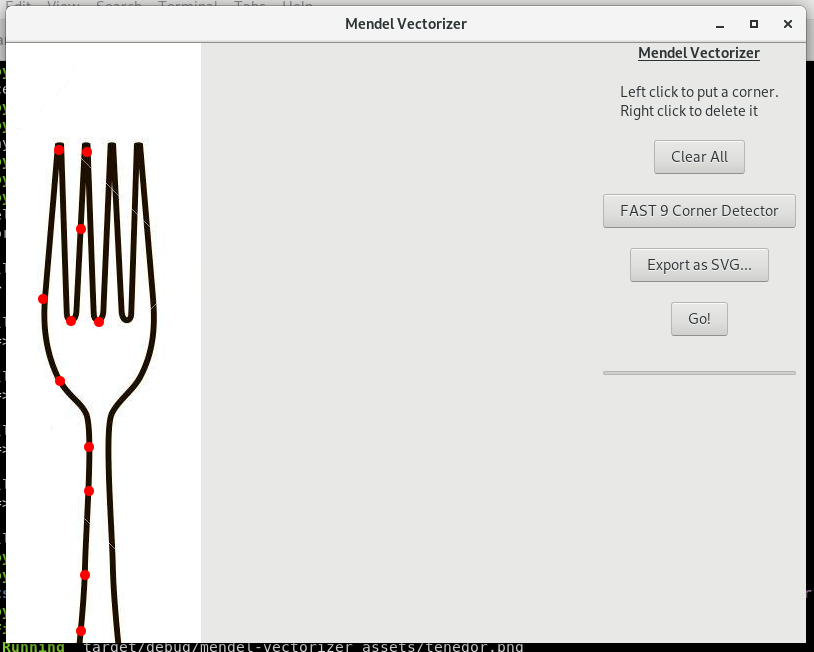
\includegraphics[width=\textwidth]{completo-fase1.png}
	}
	\caption{\label{fig:fase1} Esquinas seleccionadas en la imagen del tenedor}
\end{figure}

\begin{figure}
	\center{
		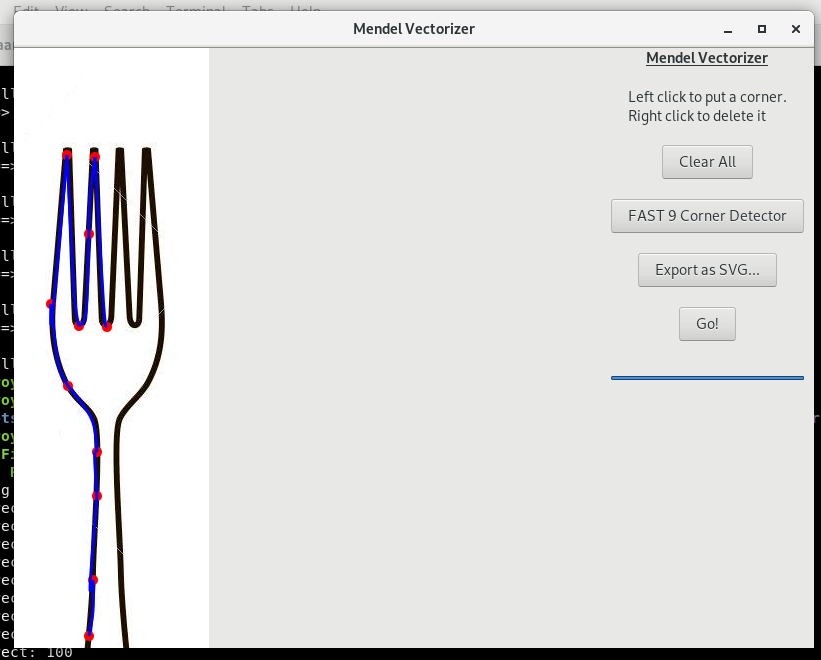
\includegraphics[width=\textwidth]{completo-fase2.png}
	}
	\caption{\label{fig:fase2} Salida del algoritmo, en azul las curvas de bézier}
\end{figure}

\begin{figure}
	\center{
		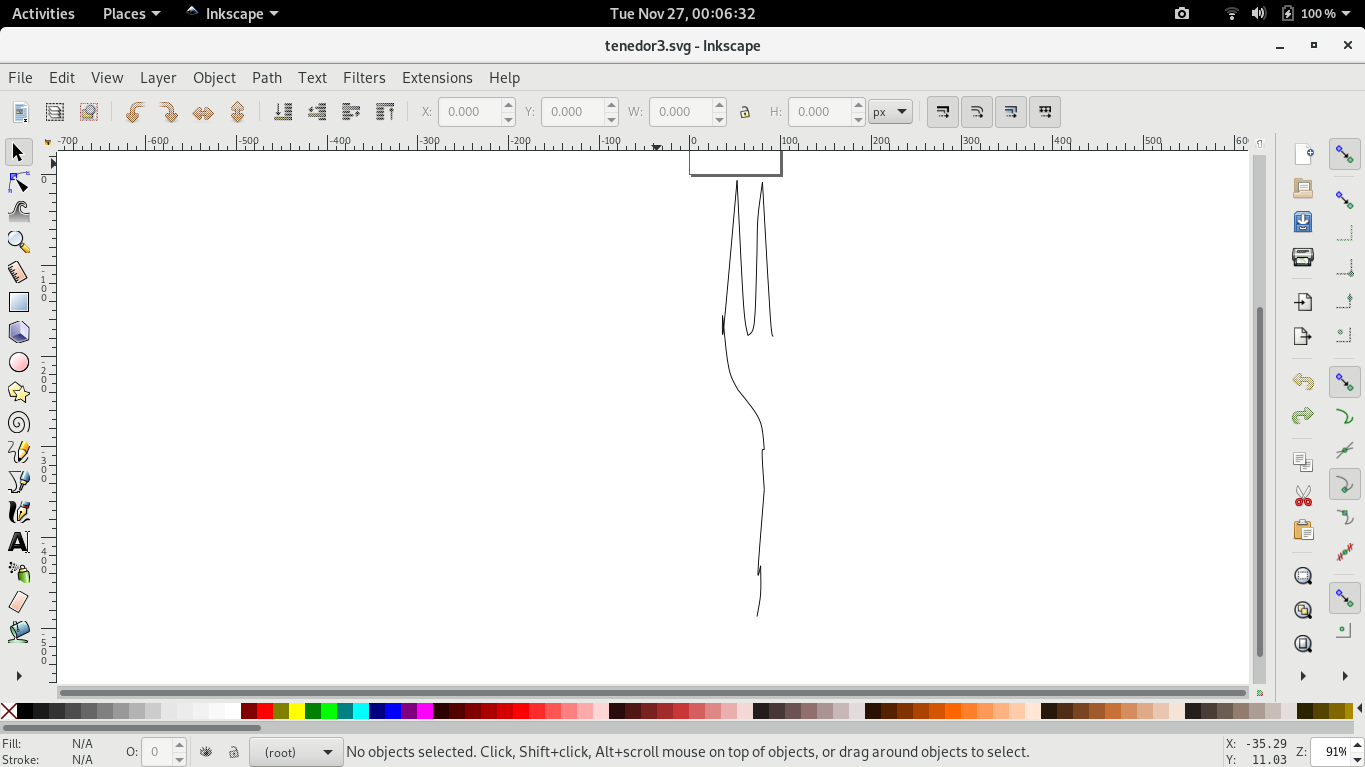
\includegraphics[width=\textwidth]{completo-fase3.png}
	}
	\caption{\label{fig:fase3} El archivo SVG generado siendo editado en Inkscape}
\end{figure}


\bibliography{memoria}
\bibliographystyle{acm}
\nocite{*}

\end{document}
